\chapter{Umsetzung und Ergebnisse}
\label{cha:umsetzung}

%Je nach Art der Arbeit kann diese Kapitelüberschrift auch \glqq Ergebnisse\grqq~lauten, z.~B. bei rein messtechnischen Aufgaben.

%Beschreibung der Umsetzung des zuvor gewählten Vorgehens (theoretische Untersuchung, Erhebungen, Durchführung von Experimenten, Prototypenaufbau, Implementierung eines Prozesses, etc.).

%Verifikation anhand der zuvor erarbeiteten Anforderungen und Validierung in Bezug auf das zuvor gestellte Ziel. Diskussion der Ergebnisse. Spätestens hier auch auf die Zuverlässigkeit der gewonnenen Erkenntnisse eingehen (z.~B. anhand der Genauigkeit von Messergebnissen).
\section{Mechanischer Aufbau des LEGO-Spike-4-Gewinnt-Roboters}


Für die Umsetzung des 4-Gewinnt-Roboters wurde eine mechanische Konstruktion gewählt, die es erlaubt, das Spielfeld zu scannen sowie Chips gezielt in eine Spalte einzuwerfen. Der Aufbau umfasst drei LEGO Spike-Motoren, einen Farbsensor und einen Drucktaster. Im Folgenden werden die einzelnen Komponenten detailliert beschrieben.

\begin{itemize}
	\item \textbf{Horizontalantrieb – Motor D}\\
	Der horizontale Antrieb des Farbsensors erfolgt über Motor D. Dieser ist dafür zuständig, die Spielfeldspalten nacheinander anzufahren. Der Motor ist mit einer Achse verbunden, welche zwei Räder antreiben. Die Bewegung erfolgt in gleichmäßigen Schritten: Eine Drehung um exakt 72 Grad bewegt den Schlitten um eine Spalte weiter. Diese Schrittweite wurde so gewählt, dass sie der Breite einer Spalte im Spielfeld entspricht. Dadurch ist eine exakte Positionierung des Sensors über jeder Spalte möglich, ohne dass zusätzliche Sensoren zur Positionsbestimmung notwendig sind. 
	\item \textbf{Vertikalantrieb – Motor E, Kette und Farbsensor}\\
	 Um das Spielfeld auch in vertikaler Richtung abfahren zu können, ist der Farbsensor an einer Kette montiert. Diese Kette wird durch Motor E angetrieben. Der Sensor ist an einem mittleren Segment der Kette befestigt und fährt beim Drehen der Kette entsprechend auf und ab. Ein Schritt des Motors um etwa 95 Grad bewegt den Sensor um genau eine Spielfeldhöhe weiter. Auf diese Weise können sämtliche sechs Reihen der aktuellen Spalte nacheinander abgescannt werden. Der Sensor wurde dabei so montiert, dass er exakt über der Mitte jedes Feldes positioniert ist, um eine zuverlässige Farberkennung zu ermöglichen. Die Rückwärtsbewegung der Kette erlaubt es, den Sensor wieder nach unten zu fahren.
	\item \textbf{Chipauswerfer – Motor A}\\
	Das Einwerfen des eigenen Spielsteins erfolgt über Motor A. An diesem Motor ist eine Stange montiert, die bei einer vollständigen Umdrehung einen Spielchip aus dem Vorratsmagazin in die gewünschte Spalte stößt. Nach der Auslösung kann ein neuer Chip in die Abschussposition nachrutschen. In der Software ist eine Wartezeit nach dem Auslösen eingebaut, damit der Chip sicher im Spielfeld ankommt, bevor die nächste Aktion beginnt.
	\item \textbf{Startsignal – Drucksensor (Force Sensor)}\\
	Um dem Roboter mitzuteilen, dass der menschliche Spieler seinen Zug abgeschlossen hat, wurde ein Drucksensor verwendet. Dieser befindet sich an der Vorderseite des Roboters. Sobald der Spieler den Sensor leicht berührt, wird ein Signal ausgelöst, das Prozess startet. 
	\item \textbf{Spielfeldscan – Farbsensor an Kette}\\
	 Für die Farberkennung des Spielfeldes wurde ein LEGO-Farbsensor verwendet, der über die oben beschriebene Kettenkonstruktion vertikal verfahrbar ist. Die Farbmessung erfolgt jeweils in der Mitte eines Spielfeldes. Der Sensor erkennt RGB-Werte, die per Software verschiedenen Spielsteinfarben (in diesem Projekt benutzt: Rot, Gelb oder Leer) zugeordnet werden. Während des Spiels vergleicht der Algorithmus die gemessenen Werte mit diesen Referenzwerten, um die tatsächliche Belegung jedes Feldes möglichst robust zu bestimmen. Der Abstand zwischen Sensor und Spielfeld beträgt etwa 7 mm – dieser Wert hat sich als optimal für zuverlässige Farbmessung erwiesen.
\end{itemize}
\textbf{Zusammenfassung}\\
Die mechanische Konstruktion basiert auf einem kartesischen Koordinatensystem, bei dem der Sensor durch die Kombination aus horizontaler (Motor D) und vertikaler Bewegung (Motor E + Kette) jede Spielfeldposition präzise anfahren kann. Das System erlaubt eine vollautomatische Spielweise: Der Roboter erkennt die aktuelle Spielsituation, berechnet den optimalen Zug und setzt diesen physisch um.


\begin{figure}[H]
	\centering
	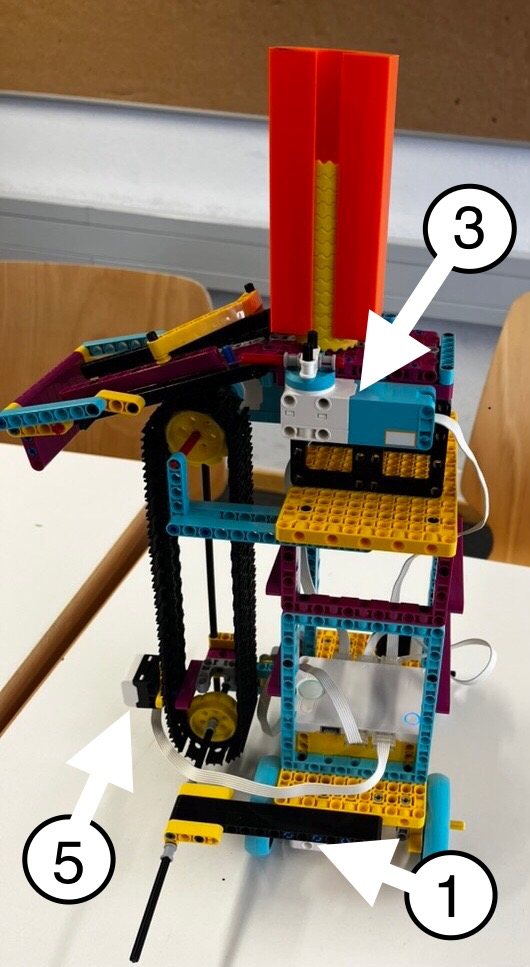
\includegraphics[width=0.5\linewidth]{images/188CF006-D571-4F2D-9337-8C4BDD7DAAEF_1_105_c}
	\caption{Seitenansicht links}
	\label{fig:188cf006-d571-4f2d-9337-8c4bdd7daaef1105c}
\end{figure}


\begin{figure}[H]
	\centering
	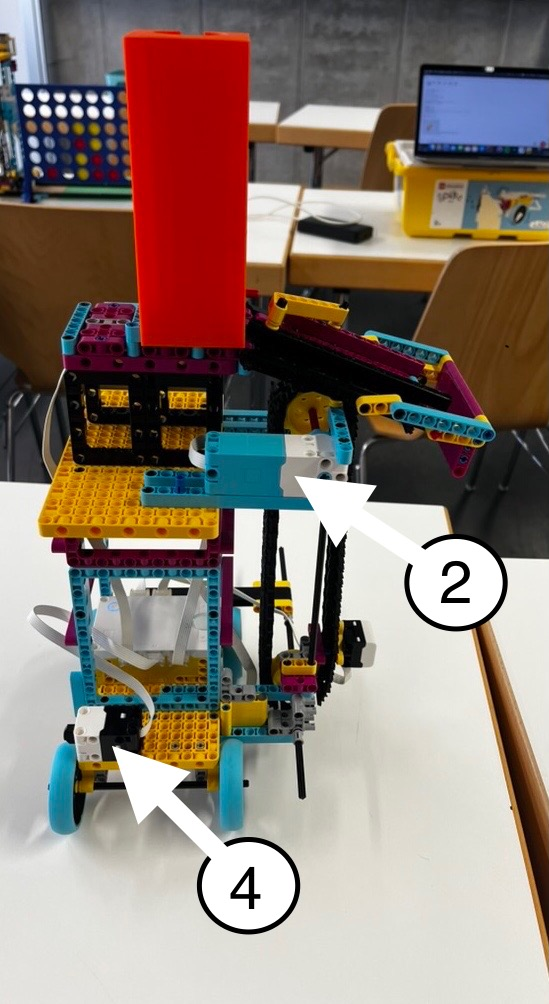
\includegraphics[width=0.5\linewidth]{images/DAE26A50-277E-4C6B-96A3-F2DE2CC9C004_1_105_c}
	\caption{Seitenansicht rechts}
	\label{fig:dae26a50-277e-4c6b-96a3-f2de2cc9c0041105c}
\end{figure}


\section{Software}
Im Kapitel Software wird genauer beschrieben, wie die Programmierung des Vier-Gewinnt-Roboters umgesetzt ist. Die Software bildet das Kernstück des Roboters und ist entscheidend dafür, dass dieser eigenständig am Spiel teilnehmen kann.



\tikzstyle{startstop} = [ellipse, draw, fill=gray!10, minimum width=3cm, minimum height=1cm]
\tikzstyle{io} = [trapezium, trapezium left angle=70, trapezium right angle=110, draw, fill=blue!10, minimum width=3cm, minimum height=1cm]
\tikzstyle{process} = [rectangle, draw, fill=orange!10, minimum width=3cm, minimum height=1cm]
\tikzstyle{decision} = [diamond, draw, fill=green!10, aspect=2, minimum width=3cm, minimum height=1cm]
\tikzstyle{arrow} = [thick,->,>=Stealth]

\begin{figure}[H]

\begin{tikzpicture}[node distance=2cm]
	\node (start) [startstop] {Start};
	\node (wait) [process, below of=start] {Warten auf Sensor-Aktivierung};
	\node (move) [process, below of=wait] {Spielfeld anfahren};
	\node (scan) [process, below of=move] {Spalten scannen};
	\node (update) [process, below of=scan] {Board-Update};
	\node (opponent) [decision, below of=update, yshift=-0.7cm] {Neuer gegnerischer Stein?};
	\node (calc) [process, below of=opponent, yshift=-0.7cm] {Optimalen Zug berechnen (Alpha-Beta)};
	\node (motor) [process, below of=calc] {Motorsteuerung: Stein platzieren};
	\node (win) [decision, below of=motor, yshift=-0.7cm] {Gewonnen?};
	\node (congrats) [startstop, right of=win, xshift=5cm] {Glückwunsch! Spiel gewonnen};
	\node (print) [process, below of=win] {Spielfeld ausgeben};

	
	\draw [arrow] (start) -- (wait);
	\draw [arrow] (wait) -- (move);
	\draw [arrow] (move) -- (scan);
	\draw [arrow] (scan) -- (update);
	\draw [arrow] (update) -- (opponent);
	\draw [arrow] (opponent) -- node[right] {Ja/Nein} (calc);
	\draw [arrow] (calc) -- (motor);
	\draw [arrow] (motor) -- (win);
	\draw [arrow] (win) -- node[above] {Ja} (congrats);
	\draw [arrow] (win) -- node[right] {Nein} (print);
	\draw [arrow] (congrats) |- (print);
	\draw [arrow] (print.west) -| ($(wait.west)+(-1.5,0)$) -- (wait.west);
	
\end{tikzpicture}

	\caption[Flussdiagramm]{Flussdiagramm der Software}
\label{fig:Flussdiagramm}
\end{figure}



\section{Algorithmus zur Entscheidungsfindung}

Ein zentraler Bestandteil des 4-Gewinnt-Roboters ist die Entscheidungsfindung durch einen algorithmischen Spielbaum. Dieser wird mit dem bekannten\newline Minimax-Algorithmus unter Verwendung von Alpha-Beta-Pruning realisiert. Ziel ist es, basierend auf dem aktuellen Spielfeldzustand den optimalen Zug für die KI zu berechnen.
Der Algorithmus bewertet mögliche Züge bis zu einer bestimmten Tiefe im Spielbaum und trifft Entscheidungen, die langfristig zum Sieg führen können oder gegnerische Gewinnzüge verhindern.

\subsection{Spielfeld und Spielerdefinition}

Im Vorfeld des Algorithmus ist festgelegt, welches Symbol der Algorithmus (die KI) spielt:

\begin{lstlisting}[style=pythonstyle]
	my_piece = 1  # 1 = YELLOW (AI player), -1 = RED
	opponent_piece = -my_piece
\end{lstlisting}

Dabei entspricht 1 dem gelben Spielstein (der KI), -1 dem roten Spielstein (dem Gegner). Diese numerische Darstellung vereinfacht die Bewertung und das Vergleichen der Felder im Spielfeld.

\subsection*{Bewertungsfunktion (evaluate)}

Der Algorithmus benötigt eine Bewertungsfunktion, die die Qualität eines Spielzustands abschätzt. Dies geschieht durch eine Heuristik, die mögliche Gewinnlinien zählt und bewertet.

Die Bewertungsfunktion basiert auf der Idee, sogenannte „Fenster“ (Ausschnitte aus 4 Feldern) im Spiel zu analysieren und zu beurteilen, wie viele Steine der KI bzw. des Gegners in diesen Fenstern enthalten sind:

\begin{lstlisting}[style=pythonstyle]
	def evaluate_window(window, player):
	opp_player = opponent_piece if player == my_piece else my_piece
	score = 0
	if window.count(player) == 4:
	score += 100
	elif window.count(player) == 3 and window.count(0) == 1:
	score += 5
	elif window.count(player) == 2 and window.count(0) == 2:
	score += 2
	if window.count(opp_player) == 3 and window.count(0) == 1:
	score -= 4
	return score
\end{lstlisting}

Diese Funktion bewertet sowohl offensive als auch defensive Situationen. Ein Fenster mit drei eigenen Steinen und einem leeren Feld wird positiv bewertet, ein Fenster mit drei gegnerischen Steinen und einem leeren Feld hingegen negativ, um Bedrohungen abzuwehren.

Die Hauptfunktion zur Bewertung des gesamten Spielfeldes aggregiert alle horizontalen, vertikalen und diagonalen Fenster:

\begin{lstlisting}[style=pythonstyle]
	def evaluate(board):
	score = 0
	center_array = [board[r][field_width//2] for r in range(field_height)]
	center_count = center_array.count(my_piece)
	score += center_count * 3
\end{lstlisting}

Zunächst werden die mittleren Spalten stärker gewichtet, da sie strategisch wichtiger sind (von dort aus können mehr Gewinnlinien entstehen).

Anschließend werden alle Zeilen, Spalten und Diagonalen analysiert:

\begin{lstlisting}[style=pythonstyle]
	for r in range(field_height):
	row_array = [board[r][c] for c in range(field_width)]
	for c in range(field_width - 3):
	window = row_array[c:c+4]
	score += evaluate_window(window, my_piece)
	score -= evaluate_window(window, opponent_piece)
\end{lstlisting}

Diese Schleifen bilden das heuristische Fundament für die spätere Entscheidungsfindung.

\subsection{Minimax mit Alpha-Beta-Pruning}

Die Hauptentscheidung trifft der Minimax-Algorithmus. Dabei wird rekursiv der Spielbaum aufgebaut, wobei sich der Algorithmus abwechselnd in die Rolle der KI („maximizing player“) und des Gegners („minimizing player“) versetzt. Um die Effizienz zu steigern, wird Alpha-Beta-Pruning genutzt. Dabei werden Äste im Spielbaum verworfen, wenn sie nachweislich zu schlechteren Ergebnissen führen.

Der Einstiegspunkt ist:

\begin{lstlisting}[style=pythonstyle]
	def alpha_beta(board, depth, alpha, beta, maximizing_player):
\end{lstlisting}

Zuerst wird geprüft, ob der aktuelle Zustand bereits im Transposition Table gespeichert ist – einem Cache zur Vermeidung redundanter Berechnungen:

\begin{lstlisting}[style=pythonstyle]
	key = (board_hash(board, maximizing_player), depth)
	if key in transposition_table:
	return transposition_table[key]
\end{lstlisting}

Anschließend erfolgt eine Terminalprüfung: Ist der Zug eine Gewinnsituation, oder wurde die maximale Tiefe erreicht?

\begin{lstlisting}[style=pythonstyle]
	valid_locations = [col for col in range(field_width) if is_valid_location(board, col)]
	terminal = winning_move(board, my_piece) or winning_move(board, opponent_piece) or len(valid_locations) == 0
	if depth == 0 or terminal:
	...
\end{lstlisting}

Falls ja, gibt die Funktion eine Bewertung zurück. Andernfalls wird der Spielbaum weiter durchlaufen.

\subsection{Maximierender Spieler (KI):}

\begin{lstlisting}[style=pythonstyle]
	if maximizing_player:
	value = -float('inf')
	for col in valid_locations:
	...
	new_score = alpha_beta(..., False)[1]
	if new_score > value:
	value = new_score
	best_col = col
	alpha = max(alpha, value)
	if alpha >= beta:
	break
\end{lstlisting}

Hier versucht der Algorithmus, die maximal erreichbare Bewertung zu finden und prüft regelmäßig, ob das aktuelle Ergebnis besser ist als die bisherige beste Option. Wenn \texttt{alpha >= beta}, wird der restliche Baum abgeschnitten (Pruning).

\paragraph*{Minimierender Spieler (Gegner):}

Analog erfolgt das Vorgehen für den Gegner:

\begin{lstlisting}[style=pythonstyle]
	else:
	value = float('inf')
	for col in valid_locations:
	...
	new_score = alpha_beta(..., True)[1]
	if new_score < value:
	value = new_score
	best_col = col
	beta = min(beta, value)
	if beta <= alpha:
	break
\end{lstlisting}

Am Ende wird das Ergebnis in der Transpositionstabelle gespeichert und zurückgegeben:

\begin{lstlisting}[style=pythonstyle]
	transposition_table[key] = result
	return result
\end{lstlisting}

\subsection{Dynamische Suchtiefe}

Je nach Spielphase kann es sinnvoll sein, tiefer oder flacher zu suchen. Zu Beginn reicht eine niedrige Tiefe, da viele Züge möglich sind. In späteren Phasen erhöht sich die Tiefe:

\begin{lstlisting}[style=pythonstyle]
	def get_dynamic_depth(board):
	empty = sum(row.count(0) for row in board)
	if empty > 30:
	return 3
	else:
	return 4
\end{lstlisting}

Diese dynamische Anpassung balanciert Spielstärke und Rechenzeit optimal.

\subsection{Fazit}

Der eingesetzte Minimax-Algorithmus mit Alpha-Beta-Pruning stellt das strategische Herzstück des 4-Gewinnt-Roboters dar. Durch gezielte Bewertung von Spielpositionen, Berücksichtigung gegnerischer Drohungen und dynamische Tiefenanpassung kann der Roboter selbstständig Züge planen, Gefahren abwehren und letztlich siegreich agieren. Die Verwendung eines Transpositionstables beschleunigt dabei die Entscheidungsfindung, indem bereits analysierte Spielsituationen nicht erneut bewertet werden müssen. Das Ergebnis ist ein hochgradig effektives Entscheidungsverfahren für ein strategisches Spiel wie 4-Gewinnt.


\subsection{Begrenzung}
Der LEGO Spike Hub besitzt mit seinem 100MHz ARM Cortex-M4 Prozessor, 320 KB RAM und 1 MB Flash-Speicher eine stark begrenzte Hardwareausstattung. Diese Ressourcen reichen für einfache Steuerungsaufgaben, setzen aber dem Einsatz komplexer Algorithmen wie Minimax enge Grenzen.

Insbesondere der geringe Arbeitsspeicher ist entscheidend: Bereits bei einer Suchtiefe von 4 erreicht der Algorithmus die Speichergrenze, da jeder Spielzug rekursiv bewertet und gespeichert wird. Eine tiefere Suche führt zu Speicherüberläufen oder langen Berechnungszeiten.

Durch Alpha-Beta-Pruning und eine dynamisch begrenzte Suchtiefe lässt sich der Algorithmus dennoch effizient auf dem Hub einsetzen – mit akzeptabler Reaktionszeit und stabiler Ausführung.